\chapter{线化小扰动方程}
\section{轴系}
\begin{enumerate}[label=\arabic*.,topsep=0pt]
\setlength{\itemsep}{-2pt}
\item Inertial Axes System $Ox_iy_iz_i$,位于地心,不随地球旋转
\item Earth-Fixed Axes System $Ox_Ey_Ez_E$,位于地心,随地球旋转
\item Navigational System $Ox_ey_ez_e$,俗称地轴系,NED坐标系
\item Body Axes System $Ox_by_bz_b$,任意一种固连与机身的坐标系,通常取体轴系
\subitem Stability axes system $Ox_sy_sz_s$,稳定性轴系,体轴系+迎角,重心-速度在对称面内方向-垂直对称面向右-向下
\subitem Wind axes system $Ox_wy_wz_w$,风轴系,体轴系+迎角+侧滑角,重心-速度方向-垂直铅垂面向右-向下

\end{enumerate}

\subsection{坐标转换}
$$
L_x(\alpha)=
\begin{pmatrix}
1&0&0\\
0&\cos\alpha&\sin\alpha\\
0&-\sin\alpha&\cos\alpha
\end{pmatrix}
L_y(\alpha)=
\begin{pmatrix}
\cos\alpha&0&-\sin\alpha\\
0&1&0\\
\sin\alpha&0&\cos\alpha
\end{pmatrix}
L_z(\alpha)=
\begin{pmatrix}
\cos\alpha&\sin\alpha&0\\
-\sin\alpha&\cos\alpha&0\\
0&0&1
\end{pmatrix}
$$

地轴系->体轴系:$L_{BE}=L_x(\phi)L_y(\theta)L_z(\psi),L_{BE}v_E=v_B$

风轴系->体轴系:$L_{BW}=L_y(\alpha)L_z(\beta),L_{BW}v_W=v_B$

\section{6自由度方程}
见SUATP

\section{线性化小扰动}
见高浩
%\begin{figure}[!h]
%\centering
%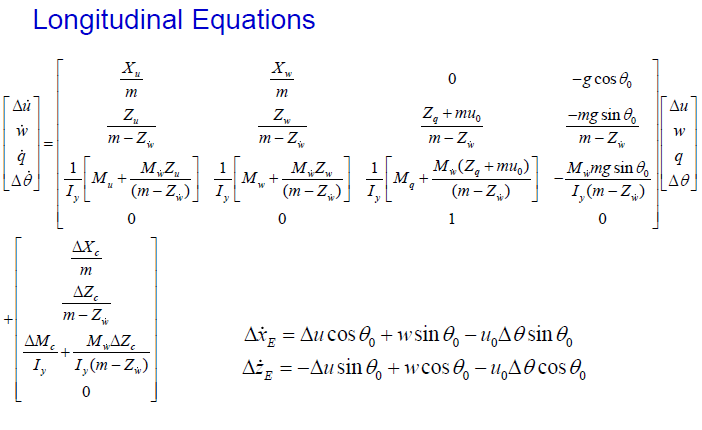
\includegraphics[width=1.1\textwidth]{loneq.png}
%\end{figure}
%\begin{figure}[!h]
%\centering
%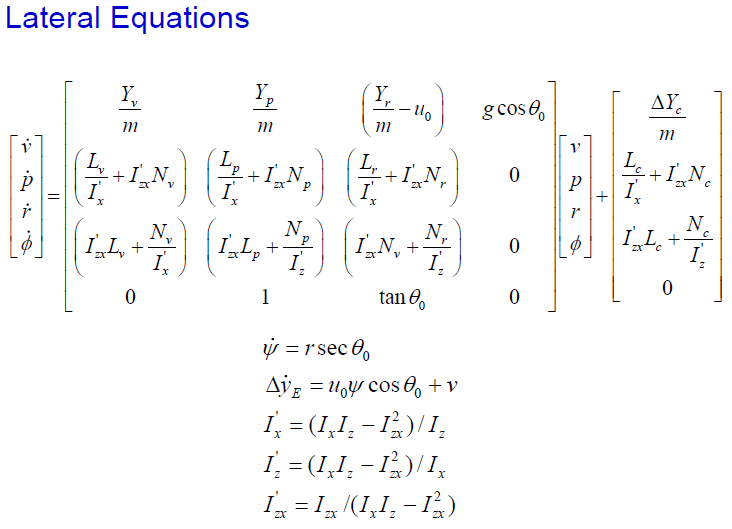
\includegraphics[width=1.1\textwidth]{lateq.png}
%\end{figure}
\endinput